\documentclass[12pt]{article}
%\documentclass[10pt, landscape, twocolumn]{article}

%\usepackage{setspace}
%\onehalfspacing
\usepackage[T2A]{fontenc}
\usepackage[utf8]{inputenc}

\usepackage[russian]{babel}

\usepackage{amsmath, amssymb}
%\usepackage[lastpage,user]{zref}

\usepackage{geometry, graphics, graphicx}

\graphicspath{ {./images/} }

\geometry
{
    a4paper,
    total={210mm,297mm},
    left=20mm,
    right=20mm,
    top=25mm,
    bottom=20mm,
}

\usepackage{hyperref}

\hypersetup{
    colorlinks=false,       % false: boxed links; true: colored links
    linkcolor=red,          % color of internal links (change box color with linkbordercolor)
    citecolor=green,        % color of links to bibliography
    filecolor=magenta,      % color of file links
    urlcolor=cyan           % color of external links
}

% ------------Колонтитулы-----------------
%\usepackage{fancyhdr}
%\pagestyle{fancy}
%
%\fancyhead{}
%\lhead{}
%\chead{}
%\rhead{}
%\lfoot{\scriptsize\textbf{UPD.:}~\emph{\today}}
%\cfoot{}
%\rfoot{\thepage /\zpageref{LastPage}}


%\usepackage{amsopn}
%\DeclareMathOperator{\B}{B}

\usepackage{hyperref}


%\usepackage{tikz}
%\usepackage{background}
%\usepackage{tikzpagenodes}
%\usepackage{lmodern}
\usepackage{indentfirst}

%\backgroundsetup%
%{   angle=0,
%    opacity=2,
%    scale=1,
%    contents=%
%    {   \begin{tikzpicture}[remember picture,scale=3]
%            \fontsize{100}{120}\selectfont
%            \node[text=gray!50,rotate=90, above=1cm] 	at (current page text area.west) {\textbf{ФН--1}};
%            \node[text=gray!50,rotate=-90, above=1cm] 	at (current page text area.east) {\textbf{ФН--1}};          
%        \end{tikzpicture}
%    }
%}
% ----------------------------------------

%\newcommand{\ul}{\underline}

%\usepackage{amsopn}
%\DeclareMathOperator{\up}{up}
%\DeclareMathOperator{\h}{h}
%\DeclareMathOperator{\fup}{fup}
%%\DeclareMathOperator{\ch}{ch}
%\DeclareMathOperator{\g}{g}

\usepackage{xcolor}
\definecolor{amaranth}{rgb}{0.9, 0.17, 0.31}
\definecolor{amethyst}{rgb}{0.6, 0.4, 0.8}
\definecolor{ao}{rgb}{0.0, 0.0, 1.0}


\title{Применение свёрточных нейронных сетей в задаче оптического распознавания текста для фильтрации нежелательных данных}
\author{Разумов Т.Е., Чуриков Д.В., Кравченко О.В.}

\begin {document}
\maketitle

\begin{abstract}
В настоящей работе решается задача построения модели для обнаружения и фильтрации нежелательных спам--сообщений. В качестве модели классификатора нежелательных писем в электронной почте выбрана полносвязная свёрточная нейронная сеть (\textsf{FCNN}). Она позволяет разделить письма на две категории: \emph{спам} и \emph{не спам}. 

Основным результатом исследования является программное приложение на языке \textsf{C++}, имеющее микро--сервисную архитектуру, и решающее задачу классификации изображений. Приложение способно выдерживать более $10^6$ запросов в минуту в режиме реального времени.
\end{abstract}


\section{Введение}
В настоящее время, объемы производимой человечеством информации
увеличиваются в геометрической прогрессии. Значительную пользу из этой информации можно извлечь лишь при правильной обработке и анализе этих данных. 

С другой стороны, актуальной задачей обработки данных является задача
фильтрации нежелательных данных, а применительно к IT--технологиям --- это задача фильтрации спам--сообщений.
Последнее связано с тем, что обмена информацией различной информации по умолчанию используется электронная почта. Электронная почта является одним из самых дешевых, простых в использовании, легкодоступных, наиболее официальных и надежных способов обмена информацией. 

Спам--сообщения, в общем случае могут содержать разнородную тестово--визуальную информацию. Алгоритмы глубокого
обучения применяются для анализа спам--писем с различной информацией, поступающих в реальном времени, в \cite{Makkar2021}.
При этом, сначала из изображения извлекаются признаки (характеристики),
а затем происходит принятие решения. 


Среди других подходов классификации можно выделить, метод опорных векторов и метод случайного леса. В работе \cite{Taylor2020} приводится сравнение этих методов для решения задачи фильтрации спам--сообщений.

Алгоритмы фильтрации являются, как правило, стохастическими \cite{Garg2021} 
и применяются в комбинации с методами оптимизации некоторой целевой функции. 
Для решения задачи классификации электронной почты применяют различные вероятностные модели. Наиболее употребимой среди них является наивный байесовский классификатор. Метод роя частиц является одним из численных методов стохастической оптимизации, его применяют в задачах фильтрации данных, так как не требуется задавать аналитическое выражение градиента оптимизируемой функции. 
Метод роя частиц относится к методам стохастической оптимизации и применяется для эвристической глобальной оптимизации параметров наивного Байесовского классификатора. Комплексный подход с использованием наивного алгоритма Байеса вместе с методом оптимизации роя частиц применялся в \cite{Parmar2020}. 
Эволюционная модель классификации спама представлена в \cite{Mohammad2020}. 

{
\bf\color{amaranth}
Добавить абзаци про задачу и её решение настоящей статьи.
}



\section{Методология}
\subsection{Формальная постановка задачи}
Пусть задано некоторое множество объектов $ X = X_L \cup X_T $, где 
$X_L$ --- обучающая выборка, 
$X_T$ --- тестовая выборка, 
$Y$ --- множество допустимых ответов. Считаем, что существует некоторая целевая функция $g: X \rightarrow Y$, значения которой известны только на множестве $X_L$. Пусть данные распределены в соответствии с некоторым неизвестным распределением $P(x,y) = P(x) P(y|x)$, при этом задана некоторая функция потерь
$$
R(g(x), y) = 
\begin{cases} 
\phantom{>}0, & y = g(x), \\
> 0, & y \neq g(x).
\end{cases}
$$

В соответствии с принципом минимизации эмпирического риска 
{\bf\color{amaranth} (что за принцип?)} нам надо минимизировать функцию потерь, то есть найти такую решающую функцию $g(x)$, которая в среднем будет приводить к наименьшей погрешности. Формально, требуется решить следующую задачу минимизации
$$
g(x) = \operatorname*{argmin}_{f: X \rightarrow Y} E_{X,Y} R(f(x), y).
$$

Для задачи фильтрации нежелательных данных множество $Y$ состоит из двух элементов $\{0, 1\}$, где $0$ и $1$ желательные и нежелательные данные соответственно. В силу грубости методов дискретных вычислений, на практике обычно используется $Y = R[0, 1]$, а результат работы классификатора $y' = g(x)$ {\bf\color{amaranth} (почему стоит штрих?)} отноcится к нужному классу с заданной пороговой вероятностью $\alpha$, минимизирующей ошибку первого и второго рода.

\subsection{Требования к решению}
В настоящее время информация перемащается с высокой скоростю, что накладывает дополнительное важное требование на скорость работы модели и системы в целом. Время проверки одного письма не должно превышать $\leqslant 3$ секунд, что наклыдвает дополнительные требования к используемым инструментам и остказоустойчивости всей системы. 

\section{Методология}

От момента получения сообщения до момента принятия решения о его типе, текстовая информация {\bf\color{amaranth} (а графическая?, про графическую расписал в разделе deploy, в конечном итоге она превращается в текстовую)} проходит через несколько этапов обработки:
\begin{enumerate}
\item Предобработка.
\item Векторизация.
\item Классификация.
\end{enumerate}

\subsection{Предобработка текста}
Поскольку текст имеет сильно неоднородную структуру и при этом одно слово может быть записано множеством разных способов (разный шрифт, кодировка, регистр итд), но при этом иметь тот же смысл, то применяются различные методы предобработки текста или их комбинация.

Первым шагом текст производится парсинг и декодирование текста в заданную кодировку. Затем приведение к нижнему (или верхнему) регистру, удаление лишних пробелов, отступов. Производится замена символов по заданному правилу. После этого применяются следующие методы:

\subsubsection*{\it\,Stop words}
Текст часто содержит много символов, которые не несут смысловой нагрузки для общего смысла (два пробела, абзацный отступ), а также стоп слова (stop words).
Стоп слова -- это слова на любом языке, которые не добавляют особого смысла предложению. 	Часто к стоп словам относят знаки пунктуации, местоимения и предлоги. Часто спамеры используют их для зашумления текстов с целью скрыть спам контент сообщения. Так как их можно спокойно игнорировать, не жертвуя смыслом предложения, то в задачах классификации часто прибегают к их удалению из исходного сообщения.

\subsubsection{\it\,Стемминг и лемматизация}
Обычно тексты содержат разные грамматические формы одного и того же слова, а также могут встречаться однокоренные слова. Используя разные алгоритмы лемматизация и стемминг преследуют цель привести все встречающиеся словоформы к одной, нормальной словарной форме.


Стемминг -- это грубый эвристический процесс, который отрезает "лишнее" от корня слов, часто это приводит к потере словообразовательных суффиксов. Основная проблема, возникающая при использовании стеммера -- это обработка слов, которые при образовании разных грамматических форм меняют не только окончание, но и основу слова. Например, существительное "кошка" в винительном и родительном падеже множественного числа имеет форму "кошек". Из-за таких беглых гласных стеммер должен либо игнорировать подобные формы, усекая "кошки" до "кошк" и теряя часть форм слова, либо усекать слово до безусловно неизменяющейся основы, получая "кош", что впоследствии может привести к полной потере контекста. Чтобы минимизировать негативные последствия слишком агрессивного усечения слов стеммером, необходимо выполнять стемминг искомого ключевого слова, а затем сравнивать результат с выходом стеммера для каждого из слов в обрабатываемом тексте. Но даже в этом случае буду встречаться совпадения стемов для совершенно несвязанных слов.


Лемматизация -- это более тонкий процесс, который использует словарь и морфологический анализ, чтобы в итоге привести слово к его канонической форме (лемме). Однако он применяет упрощенный анализ слов, не учитывая контекст. Это приводит к неоднозначностям при определении части речи. Например, лемматизация слов в словосочетании "мы роем яму" даст для второго слова два варианта лемматизации: существительное рой и глагол рыть. Эта неоднозначность не может быть разрешена без привлечения морфологического анализатора.

Как правило лемматизация дает наиболее точные результаты и именно этот подход используется в работе.

\subsection{Векторизация текста}
Современные алгоримы машинного обучения не могут напрямую работать с сырым текстом, поэтому необходимо построить отображение текста в векторное пространство. Это называется извлечением признаков. Рассмотрим несколько подходов для построения данного отображения.

\subsubsection*{\it\,Мешок слов}
Модель "мешок слов" - это упрощенное представления текстовой информации, используемое в задачах обработки естественных языков и поиска информации. В этой модели текст представляется в виде мешка (мультимножества) его слов или словосочетаний в случае комбинаций термов, игнорируя грамматику и в некоторых случаях даже порядок слов, но сохраняя множественность. Каждому такому терму (слову или словосочетанию) ставится в соответствие некоторое число. В этом случае текст определяется вектором $x=(x_1, ..., x_N)^T$, где $N$ - размерность из конечного словаря $X_L$ состоящего из уникальных термов обучающей выборки. Возможны следующие варинаты определения $x_i$
\begin{itemize}
\item Булевский вес: $\begin{cases} 1, & \mbox{если элемент присутствует в письме} \\ 0, & \mbox{если элемент не присутствует в письме}  \end{cases}$
\item Количество вхождений i-го терма в тексте: $x_i = n_i$
\item Частота терма: $x_i = \dfrac{n_i}{\sum n_k}$
\end{itemize}

В данной работе для определения $x_i$ мы взяли частоту терма.

\subsubsection*{\it\,Word2Vec}

\subsubsection*{\it\,Fast Text}

\subsection*{Классификация текста}
После векторизации текста мы должны построить преобразование из множества признаков во множество классифицируемых объектов $g: X \rightarrow Y$

\subsubsection*{\it\,Оценка порога принятия решения}
Согласно статье [twitter threshold p. 4.6] для того чтобы выбрать порог принятия рещений классификатора, который минимизует дисперсии оценок точности, выведена следующая формула:

На основе которой была произведена разметка и вычеслена оптимальная пороговая точность $\alpha = 0.75$. 

\subsubsection*{\it\,Логистическая регрессия}
Наиболее частым методом используемым в задаче классификации используется метод логистической регрессии:
$$
g(x) = \left(1 + \exp{ \left( \sum_{i=0}^n w_i x_i  \right) }\right)^{-1},
$$
где $w=(w_1, ..., w_N)^T$ --- веса модели, полученные при обучении.

Приведем результаты расчетов для разных способов векторизации текста.

Для BOW эмбедингов мы имеем следующие результаты:
\begin{center}
  \begin{tabular}{ | c | c | c |}
    \hline
     precision & recall & accuracy \\ \hline
     0.91143 & 0.99961 & 0.93395 \\ \hline
  \end{tabular}
\end{center}


Для Fast Text эмбедингов мы имеем следующие результаты:
\begin{center}
  \begin{tabular}{ | c | c | c |}
    \hline
     precision & recall & accuracy \\ \hline
     0.95523 & 0.8916 & 0.9371  \\ \hline
  \end{tabular}
\end{center}

\subsubsection*{\it\,Fully convolutional neural network}

Fully convolutional neural network для нашей задачи имеет 3 слоя. На первых двух используется функция активации $ReLU$, на последнем $Sigmoid$. На каждом слое производится регуляризация данных. В нашем случе нейронную сеть можно определить формулой:

$$
g(x) = h_2 \left(\sum_{k=0}^{n_2} w''_k h_1\left(\sum_{j=0}^{n_1} w'_j h_0\left( \sum_{i=0}^{n_0} w_i x_i \right)\right)\right)
$$

где $h_i$ -- функция активации для соответствующего слоя.

Для BOW эмбедингов мы имеем следующие результаты:
\begin{center}
  \begin{tabular}{ | c | c | c |}
    \hline
     precision & recall & accuracy \\ \hline
     0.93604 & 0.95643 & 0.93764 \\ \hline
  \end{tabular}
\end{center}

Для Fast Text эмбедингов мы имеем следующие результаты:
\begin{center}
  \begin{tabular}{ | c | c | c |}
    \hline
     precision & recall & accuracy \\ \hline
     0.99931 & 0.9126 & 0.98476 \\ \hline
  \end{tabular}
\end{center}

\subsection{Аспекты реализации алгоритмов}

\subsubsection*{\it\,Микросервисная архитектура}

Поскольку сервис должен работать под высокими нагрузками важно обеспечить архитектуру, при которой выход из строя одной компоненты не приведет к деградации всей системы. Реализована следующая клиент-серверная архитектура (рис. 1). Antispam daemon (mrasd) парсит входящие сообщение и извлекает оттуда текст, изображения, pdf.  Поскольку нежелательные данные часто содержатся внутри вложенных изображений и документов, то из них также необходимо извлечь текст. Для этого через отложенную redis очередь документы оправляются в OCR сервис, который извлекает текст и сохраняет результат в redis cache.

Так как, с большой вероятностью письмо может быть дубликатом (например в случае ddos атаки или оффлайн перепроверки), то чтобы не нагрузать лишний раз OCR сервис, производится первичная проверка redis cache на наличие уже обработанных данных по заданному хэшу документа.

После полного извлечения текста сервис mrasd производит все этапы предобработки текста (приведение к одному регистру, удаление стоп слов, нормализация), а затем отправляет текст в сервис mlapi по протоколу grpc для векторизации текста при помощи fast text и дальнейшего получения предсказания fcnn модели по котому принимается решение о "нежелательности"  входящего сообщения.

Предложенная архитектура хороша тем, что при выходе из строя OCR сериса, одного (или нескольких) инстансов redis сluster, не деградирует вся система в целом.
 
\begin{figure}[h!]
	\center
	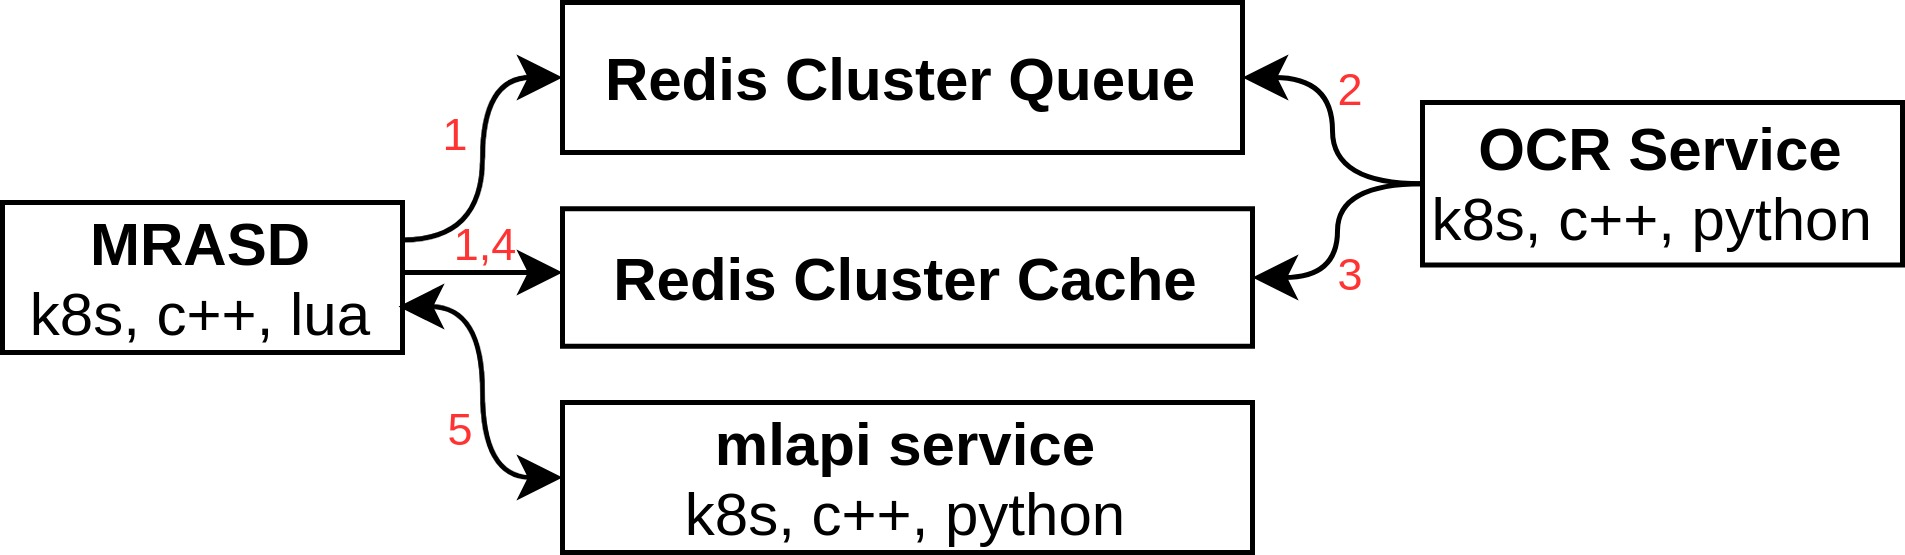
\includegraphics[scale=0.25]{deploy.jpg}
	\caption{Deploy}
	\label{fig:02}
\end{figure}


\begin{figure}[h!]
	\center
	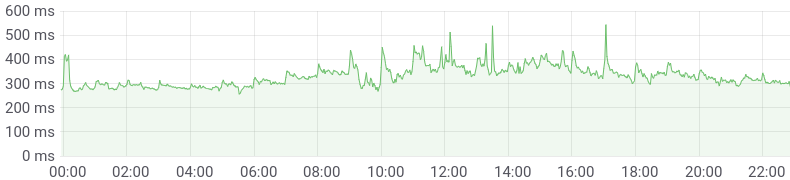
\includegraphics[scale=0.25]{timings.png}
	\caption{Среднее время обработки письма}
	\label{fig:03}
\end{figure}


\begin{figure}[h!]
	\center
	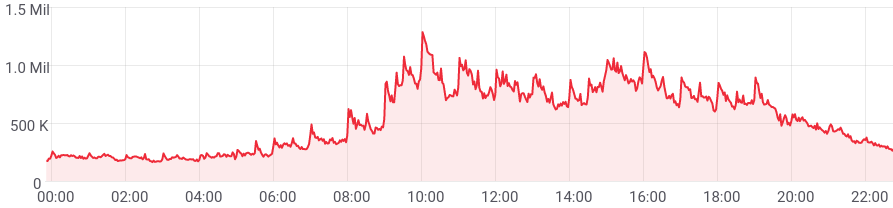
\includegraphics[scale=0.25]{processed_messages.png}
	\caption{Среднее количество запросов в минуту с одной из ферм}
	\label{fig:04}
\end{figure}

\subsubsection*{\it\,Обзор библиотек}

Поскольку от сервисов требуется высокая производительность, то для его написания выбран язык C++ (stl17, grpc, boost), как один из самых производительных современных языков. Для анализа данных и обучения fcnn модели использовался язык Python3 и фреймврок pyTorch за счет высокой производительности и возможности проведения параллельных вычислений, как на cpu, так и на gpu ядрах машины.

Отказоустойчивость всех наших микросервисов обеспечивается за счет их развертки в k8s, так как внутри него можно настроить: автоматическую балансировку нагрузки с помощью постоянного мониторинга сведений о производительности и использовании ресурсов; грамотное размещение подов внутри кластера по дата центрам (правило affinity); при падении любого пода по какой-либо причине запросы равномерно сбалансируются по оставшимся живым подам, до тех пор, пока k8s сам их не переподнимет.


\section{Conclusions}
{
\bf\color{amaranth}
Решены следующие задачи
\begin{enumerate}
	\item \ldots
	\item \ldots
	\item \ldots
\end{enumerate}

Получены следующие результаты
\begin{enumerate}
\item \ldots
\item \ldots
\item \ldots
\end{enumerate}
}

\begin{thebibliography}{99}
\bibitem{Makkar2021} 
Aaisha Makkar, Uttam Ghosh, Pradip Kumar Sharma.
2021. \emph{Artificial Intelligence and Edge Computing-enabled
	Web Spam Detection for Next Generation IoT
	Applications} // IEEE Sensors Journal

\bibitem{Taylor2020}
Taylor O.E., Ezekiel P.S.
2020. \emph{A Model to Detect Spam Email Using Support Vector Classifier and Random Forest Classifier} //
International Journal of Computer Science and Mathematical Theory

\bibitem{Garg2021}
Pranjul Garg, Nancy Girdhar.
2021. \emph{A systematic review on spam filtering techniques based on
natural language processing framework} // 2021 11th International Conference on Cloud Computing, Data Science \& Engineering (Confluence 2021)

\bibitem{Parmar2020}
Nandan Parmar, Ankita Sharma, Harshita Jain, Amol K. Kadam.
2020. \emph{Email Spam Detection using Naïve Bayes and Particle Swarm Optimization} // IJIRT

\bibitem{Mohammad2020}
Rami Mustafa A. Mohammad.
2020. \emph{A lifelong spam emails 	classification model} //
Applied Computing and Informatics
\end{thebibliography}



\end {document}
